\documentclass{beamer}

\usepackage{graphicx}
\usepackage{amsmath}
\usepackage{framed}

\begin{document}
	% = http://cran.rstudio.com/web/packages/dplyr/vignettes/introduction.html
\begin{frame}[fragile]
\frametitle{dplyr : Grammar of data manipulation}
\textbf{What is dplyr?}
\begin{itemize}
	\item dplyr is mainly authored by Hadley Wickham and Romain Francois. It is designed to be intuitive and easy to learn, thereby making ``doing things" in \texttt{R} more user-friendly.
	\item dplyr is a new package which provides a set of tools for efficiently manipulating datasets in \texttt{R}.
	\item dplyr is the next iteration of plyr, focussing on only data frames. \item dplyr is faster, has a more consistent API and should be easier to use. 
\end{itemize}
\end{frame}
%=================================================================== %

\begin{frame}
\frametitle{dplyr : abstract by Hadley Wickham}	
\textbf{Hadley Wickham's Abstract}\\
	\noindent There are three key ideas that underlie dplyr:
	
	\begin{enumerate}
		\item[1] Your time is important, so Romain Francois has written the key pieces in \textbf{Rcpp} to provide blazing fast performance. \\ \bigskip Performance will only get better over time, especially once we figure out the best way to make the most of multiple processors. 
\end{enumerate}
\end{frame}
%========================================================== %
\begin{frame}
\frametitle{dplyr : abstract by Hadley Wickham}	

\begin{enumerate}
		\item[2] Tabular data is tabular data regardless of where it lives, so you should use the same functions to work with it. \\ \bigskip
		
		With dplyr, anything you can do to a local data frame you can also do to a remote database table. \\ \bigskip PostgreSQL, MySQL, SQLite and Google bigquery support is built-in; adding a new backend is a matter of implementing a handful of S3 methods. 
\end{enumerate}
\end{frame}
%========================================================== %
\begin{frame}
\frametitle{dplyr : abstract by Hadley Wickham}	

	\begin{enumerate}
		\item[3] The bottleneck in most data analyses is the time it takes for you to figure out what to do with your data
		\\ \bigskip \textbf{dplyr} makes this easier by having individual functions that correspond to the most common operations  (\texttt{group\_by}, \texttt{summarise},\texttt{mutate}, \texttt{filter}, \texttt{select} and \texttt{arrange}). 	\\ \bigskip Each function does one only thing, but does it well.
	\end{enumerate}
\end{frame}
%======================================================================================= %

\begin{frame}
	
	\frametitle{Working with dplyr} \textbf{dplyr} focussed on tools for working with data frames (hence the \textbf{d} in the name). 

\textbf{dplyr} has three main goals:
\begin{itemize}
	\item Identify the most important data manipulation tools needed for data analysis and make them easy to use from \texttt{R}.
	
	\item Provide very fast performance for in-memory data by writing key pieces in C++.
	
	\item Use the same interface to work with data no matter where it's stored, whether in a data frame, a data table or database.
\end{itemize}
\end{frame}
%\subsection{Installing dplyr}
%You can install the latest released version from CRAN with the code below.
%You can also install and load the data packages used in most examples: 
%\begin{framed}
%	\begin{verbatim}
%	install.packages("dplyr")
%	install.packages(c("nycflights13", "Lahman"))
%	
%	library(dplyr) # for functions
%	library(nycflights13) # for data
%	\end{verbatim}
%\end{framed}
%===================================================================== %
\begin{frame}
\frametitle{Tidy Data}
\begin{itemize}

\item To make the most of dplyr, Hadley Wickham recommends that you familiarise yourself with the \textbf{principles of tidy data}. 
\item This will help you get your data into a form that works well with \textbf{dplyr}, \textbf{ggplot2} and \texttt{R}'s many modelling functions.
\end{itemize}
\end{frame}

%====================================================================== %
\begin{frame}[fragile]
\begin{framed}
	\noindent Three Principles from Hadley Wickham's paper
	\begin{itemize}
		\item[1.] Each variable forms a column, 
		\item[2.] Each observation forms a row, 
		\item[3.] Each table/file stores data about one kind of observation.
	\end{itemize}
\end{framed}
\noindent \textbf{Remark:} \\  The paper ``\textit{\textbf{Tidy data}}" by Hadley Wickham (RStudio) can be downloaded from 
\begin{verbatim}
http://vita.had.co.nz/papers/tidy-data.pdf
\end{verbatim}
\end{frame}
%=================================================================== %
\begin{frame}
\frametitle{Key data structures}

The key object in \textbf{dplyr} is a \texttt{tbl}, a representation of a tabular data structure. Currently dplyr supports:

\begin{itemize}
	\item data frames - the  most commonly encountered R data structure. 
	\item data tables - a data structure that is designed for intensive data analysis.
\end{itemize}

%\noindent For this class, We will concentrate on \textbf{dplyr} exercises with data frames mostly. However we would advise you to try and learn more about working with data tables in the future.\\
%\bigskip
\end{frame}
%============================================================================= %
\begin{frame}
	\textbf{Advances Database Users}\\
\noindent For advanced users, \textbf{dplyr} also supports the following databases: \textit{SQLite, PostgreSQL, Redshift, MySQL/MariaDB, Bigquery, MonetDB} and data cubes with arrays (partial implementation).\\ \bigskip We will not cover those topics in this workshop.
\end{frame}
%============================================================================= %
\begin{frame}
	\frametitle{CRAN tutorial}
\begin{figure}
\centering
\includegraphics[width=1.15\linewidth]{"introdplyr"}

\end{figure}

\end{frame}
%=======================================================================================%
\begin{frame}[fragile]
\frametitle{Installing dplyr}
Straightforward R package installation.
\begin{framed}
\begin{verbatim}
install.packages("dplyr")
library(dplyr)

# Data Set Examples
# 1. iris
# 2. mtcars

\end{verbatim}
\end{framed}
\end{frame}
%===================================================================== %
	
	\begin{frame}[fragile]
		\frametitle{iris data set}
\begin{framed}
		\begin{verbatim}
		> names(iris)
		[1] "Sepal.Length"
		[2] "Sepal.Width" 
		[3] "Petal.Length"
		[4] "Petal.Width" 
		[5] "Species"    
		\end{verbatim}
\end{framed}
	\end{frame}
%============================================================================ %

\begin{frame}[fragile]
\frametitle{mtcars data set}
\begin{framed}
\begin{verbatim}
> names(mtcars)
[1] "mpg"  "cyl"  "disp" "hp"  
[5] "drat" "wt"   "qsec" "vs"  
[9] "am"   "gear" "carb"
\end{verbatim}
\end{framed}
\end{frame}
%===================================================================================%
\begin{frame}[fragile]
\frametitle{Example Data Sets}
\begin{framed}
	\begin{verbatim}
		dim(iris)
		[1] 150   5
		class(iris)
		[1] "data.frame"
		mode(iris)
		[1] "list"
		
		dim(mtcars)
		[1] 32 11
		class(mtcars)
		[1] "data.frame"
		mode(mtcars)
		[1] "list"
	\end{verbatim}
\end{framed}
\end{frame}
%MAM: Maybe present tbl here! Using as.tbl on iris or mtcar
%==================================================================================== %
\begin{frame}[fragile] % You can emphasize that it's so big it can't display!
\frametitle{Data frame can be problematic}
\begin{framed}
\vspace{-6mm} 		
	\begin{verbatim}
		> mtcars
                     mpg cyl  disp  hp drat    wt  qsec vs am gear carb
Mazda RX4           21.0   6 160.0 110 3.90 2.620 16.46  0  1    4    4
Mazda RX4 Wag       21.0   6 160.0 110 3.90 2.875 17.02  0  1    4    4
Datsun 710          22.8   4 108.0  93 3.85 2.320 18.61  1  1    4    1
Hornet 4 Drive      21.4   6 258.0 110 3.08 3.215 19.44  1  0    3    1
Hornet Sportabout   18.7   8 360.0 175 3.15 3.440 17.02  0  0    3    2
Valiant             18.1   6 225.0 105 2.76 3.460 20.22  1  0    3    1
Duster 360          14.3   8 360.0 245 3.21 3.570 15.84  0  0    3    4
Merc 240D           24.4   4 146.7  62 3.69 3.190 20.00  1  0    4    2
Merc 230            22.8   4 140.8  95 3.92 3.150 22.90  1  0    4    2
Merc 280            19.2   6 167.6 123 3.92 3.440 18.30  1  0    4    4
Merc 280C           17.8   6 167.6 123 3.92 3.440 18.90  1  0    4    4
Merc 450SE          16.4   8 275.8 180 3.07 4.070 17.40  0  0    3    3
Merc 450SL          17.3   8 275.8 180 3.07 3.730 17.60  0  0    3    3
Merc 450SLC         15.2   8 275.8 180 3.07 3.780 18.00  0  0    3    3
Cadillac Fleetwood  10.4   8 472.0 205 2.93 5.250 17.98  0  0    3    4
Lincoln Continental 10.4   8 460.0 215 3.00 5.424 17.82  0  0    3    4
Chrysler Imperial   14.7   8 440.0 230 3.23 5.345 17.42  0  0    3    4
Fiat 128            32.4   4  78.7  66 4.08 2.200 19.47  1  1    4    1
Honda Civic         30.4   4  75.7  52 4.93 1.615 18.52  1  1    4    2
Toyota Corolla      33.9   4  71.1  65 4.22 1.835 19.90  1  1    4    1
Toyota Corona       21.5   4 120.1  97 3.70 2.465 20.01  1  0    3    1
Dodge Challenger    15.5   8 318.0 150 2.76 3.520 16.87  0  0    3    2
AMC Javelin         15.2   8 304.0 150 3.15 3.435 17.30  0  0    3    2
Camaro Z28          13.3   8 350.0 245 3.73 3.840 15.41  0  0    3    4
Pontiac Firebird    19.2   8 400.0 175 3.08 3.845 17.05  0  0    3    2
Fiat X1-9           27.3   4  79.0  66 4.08 1.935 18.90  1  1    4    1
Porsche 914-2       26.0   4 120.3  91 4.43 2.140 16.70  0  1    5    2
Lotus Europa        30.4   4  95.1 113 3.77 1.513 16.90  1  1    5    2
Ford Pantera L      15.8   8 351.0 264 4.22 3.170 14.50  0  1    5    4
Ferrari Dino        19.7   6 145.0 175 3.62 2.770 15.50  0  1    5    6
Maserati Bora       15.0   8 301.0 335 3.54 3.570 14.60  0  1    5    8
Volvo 142E          21.4   4 121.0 109 4.11 2.780 18.60  1  1    4    2
	\end{verbatim}
\end{framed}
\end{frame}
%==================================================================================== %
\begin{frame}[fragile] % Much nicer
\frametitle{tbl can be much better}
\begin{framed}
\vspace{-6mm} 		
	\begin{verbatim}
> mtcars <- as.tbl(mtcars)
> mtcars
Source: local data frame [32 x 11]
    mpg cyl  disp  hp drat    wt  qsec vs am
1  21.0   6 160.0 110 3.90 2.620 16.46  0  1
2  21.0   6 160.0 110 3.90 2.875 17.02  0  1
3  22.8   4 108.0  93 3.85 2.320 18.61  1  1
4  21.4   6 258.0 110 3.08 3.215 19.44  1  0
5  18.7   8 360.0 175 3.15 3.440 17.02  0  0
6  18.1   6 225.0 105 2.76 3.460 20.22  1  0
7  14.3   8 360.0 245 3.21 3.570 15.84  0  0
8  24.4   4 146.7  62 3.69 3.190 20.00  1  0
9  22.8   4 140.8  95 3.92 3.150 22.90  1  0
10 19.2   6 167.6 123 3.92 3.440 18.30  1  0
..  ... ...   ... ...  ...   ...   ... .. ..
Variables not shown: gear (dbl), carb (dbl)
\end{verbatim}
\vspace{-6mm} 		
\end{framed}
\end{frame}
%==================================================================================== %
\begin{frame}
\frametitle{dplyr; Single Table Verbs}
\textbf{dplyr} aims to provide a function for each basic verb of data manipulating:
\begin{itemize}
	\item \texttt{ filter() } (and \texttt{  slice() })
	\item \texttt{ arrange() }
	\item \texttt{ select() } (and \texttt{  rename() })
	\item \texttt{ distinct() }
	\item \texttt{ mutate() } (and \texttt{  transmute() })
	\item \texttt{ summarise() }
	\item \texttt{ sample\_n() } and \texttt{  sample\_frac() }
\end{itemize}
%	\begin{figure}
%\centering
%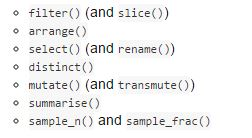
\includegraphics[width=0.7\linewidth]{singletableverbs}
%
%\end{figure}
\end{frame}
%================================================================================ %
\begin{frame}
\frametitle{Grouped operations}
\begin{itemize}

\item The verbs are useful, but they become really powerful when you combine them with the idea of “group by”, repeating the operation individually on groups of observations within the dataset. 
\item In \textbf{dplyr}, you use the \texttt{group\_by()} function to describe how to break a dataset down into groups of rows. 
\item You can use the resulting object in the same functions as above; they'��ll automatically work 'by group'� when the input is a grouped.
\end{itemize}
\end{frame}

\begin{frame}
%======================================================================================%
\frametitle{\texttt{group\_by }}

Group a tbl by one or more variables.\\ \bigskip

\textbf{Description}\\ \bigskip

Most data operations are useful done on groups defined by variables in the the dataset. The
\textbf{group\_by} function takes an existing tbl and converts it into a grouped tbl where operations are
performed "by group".

\end{frame}
%=========================================================== %
\begin{frame}
\frametitle{Summary Statistics}
You use \texttt{summarise()} with aggregate functions, which take a vector of values, and return a single number.\\ \bigskip There are many useful functions in base R like \texttt{min()}, \texttt{max()}, \texttt{mean()}, \texttt{sum()}, \texttt{sd()}, \texttt{median()}, and \texttt{IQR()}.\\ \bigskip dplyr provides a handful of others:
\begin{itemize}
\item 
\texttt{n()}: number of observations in the current group
\item 
\texttt{n\_distinct(x)}: count the number of unique values in x.
\end{itemize}

%
%first(x), last(x) and nth(x, n) - these work similarly to x[1], x[length(x)], and x[n] but give you more control of the result if the value isn’t present.
\end{frame}
%=========================================================================================%
% MAM: I've added the code in, it's nicer... you could start to use knitr! It would make this really easy!
\begin{frame}[fragile]
\frametitle{Grouping with the \texttt{group\_by} command}
\begin{framed}
\vspace{-6mm} 	
\begin{verbatim}	
> iris.sp <- group_by(iris,Species)
> class(iris.sp)
[1] "grouped_df" "tbl_df"   "tbl"    "data.frame"
		
> summarise(iris.sp,mean(Sepal.Length),
          sd(Petal.Length))
          
Source: local data frame [3 x 3]

     Species mean(Sepal.Length) sd(Petal.Length)
1     setosa              5.006        0.1736640
2 versicolor              5.936        0.4699110
3  virginica              6.588        0.5518947
\end{verbatim}
\vspace{-6mm} 	
\end{framed}
\end{frame}
%==================================================================== %
%\begin{frame}
%\begin{figure}
%\centering
%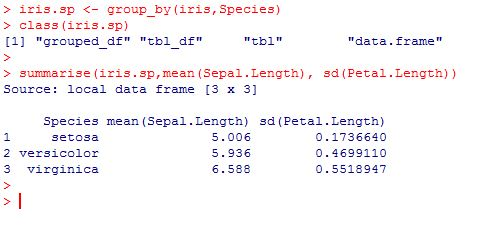
\includegraphics[width=1.05\linewidth]{irisgroupby}
%\end{figure}
%\end{frame}	

%============================================================================== %
\begin{frame}
\begin{figure}
\centering
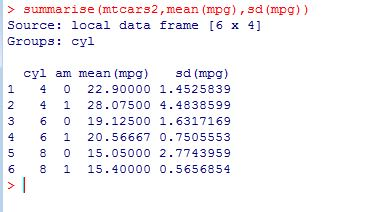
\includegraphics[width=1.1\linewidth]{mtcarssummarise}
\label{fig:mtcarssummarise}
\end{figure}
\end{frame}
		
	
%=========================================================================================%
\begin{frame}
\frametitle{Filter rows with \texttt{filter()}}
\begin{itemize}
\item \texttt{filter()} allows you to select a subset of the rows of a data frame. 
\item The first argument is the name of the data frame, and the second and subsequent are filtering expressions evaluated in the context of that data frame.
\end{itemize}



\end{frame}
%=========================================================================================%
\begin{frame}[fragile]	
\begin{framed}
\begin{verbatim}
	# Species is Virginica
	> iris.vir1 <- filter(iris,Species=="virginica")
	
	# Species is Virginica OR Petal.length > 3.2
	> iris.vir2 <- filter(iris,
	     Species=="virginica" | Petal.Length > 3.2)
	
	# Species is Virginica AND Petal.length > 3.9
	> iris.vir3 <- filter(iris,
	     Species=="virginica" & Petal.Length > 3.9)
	
\end{verbatim}
\end{framed}
\end{frame}
%========================================================================================%
\begin{frame}
\frametitle{Ordering Data Sets with \texttt{arrange()}}
\begin{itemize}
\item \texttt{arrange()} works similarly to \texttt{filter()} except that instead of filtering or selecting rows, it reorders them. 

\item It takes a data frame, and a set of column names (or more complicated expressions) to order by.

\item If you provide more than one column name, each additional column will be used to break ties in the values of preceding columns.

\item Use \texttt{desc()} (or \texttt{rev()}) to order a column in descending order.

%arrange(flights, desc(arr_delay))
\end{itemize}
\end{frame}
%===================================================================================== %
\begin{frame}
	\begin{figure}
		\centering
		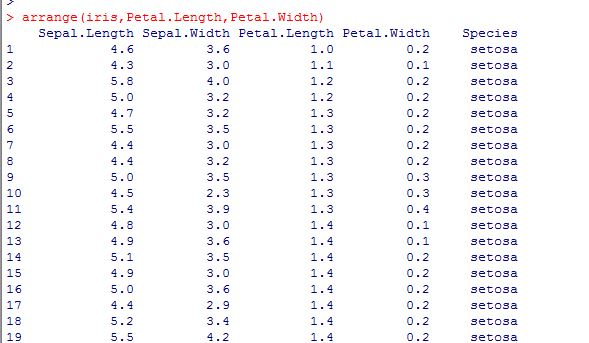
\includegraphics[width=0.97\linewidth]{irisarrange}
		
	\end{figure}
	
\end{frame}

%==================================================================================== %

\begin{frame}
	\begin{figure}
		\centering
		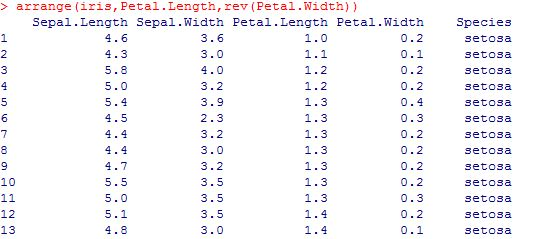
\includegraphics[width=0.97\linewidth]{irisarrange2}
		
	\end{figure}
	
\end{frame}

% Graphics: irisarrange

%=====================================================================================%
\begin{frame}
\frametitle{Select columns with \texttt{select()}}
\begin{itemize}
\item Often you have a dataset with many columns of which only a few are of interest to you. 
\item \texttt{select()} allows you to rapidly zoom in on a useful subset using operations that usually only work on numeric variable positions.
\end{itemize}
\end{frame}
%=====================================================================================%
\begin{frame}
\frametitle{Selection Options with \texttt{select()}}
\begin{figure}
\centering
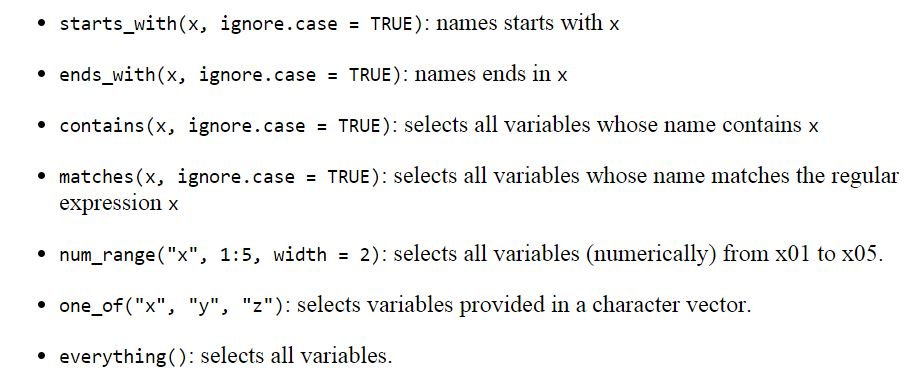
\includegraphics[width=01.05\linewidth]{selectoptions}
\end{figure}
\end{frame}
%=====================================================================================%
\begin{frame}
	\frametitle{Selection Options with \texttt{select()}}
	
	\begin{figure}
		\centering
		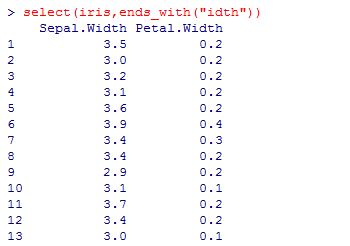
\includegraphics[width=0.69\linewidth]{selectendswith}
	\end{figure}
\end{frame}
%=====================================================================================%
\begin{frame}
\frametitle{Selection Options with \texttt{select()}}

\begin{figure}
\centering
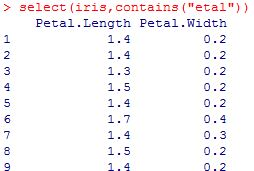
\includegraphics[width=0.69\linewidth]{selectioncontaints}
\end{figure}
\end{frame}
%=====================================================================================%
\begin{frame}
\frametitle{Sampling rows with \texttt{sample\_n()} and \texttt{sample\_frac()}}
\begin{itemize}
\item Use \texttt{sample\_n()} and \texttt{sample\_frac()} to take a random sample of rows
\begin{itemize}
\item Fixed number for \texttt{sample\_n()} 
\item Fixed fraction for \texttt{sample\_frac()}.
\end{itemize}
\end{itemize}
\end{frame}
%=====================================================================================%
% MAM: show smaller example, n=2 so they can get more out of the printed results
\begin{frame}[fragile]
\frametitle{Sampling rows with \texttt{sample\_n()}}
\begin{framed}
\vspace{-6mm} 	
\footnotesize{
\begin{verbatim}
# Sample 2 row from iris
> sample_n(iris, 2)
Source: local data frame [2 x 5]

  Sepal.Length Sepal.Width Petal.Length Petal.Width   Species
1          6.3         2.7          4.9         1.8 virginica
2          5.1         3.5          1.4         0.3    setosa	
\end{verbatim}
}
\vspace{-6mm} 	
\end{framed}
\end{frame}
%=====================================================================================%
% Show the grouped object after the smaple_n
\begin{frame}[fragile]
\frametitle{Sampling rows with \texttt{sample\_n()} on a grouped object}
\begin{framed}
\vspace{-6mm} 
\footnotesize{
\begin{verbatim}
# Sample 2 row per species
# iris.sp is a grouped object
> class(iris.sp)
[1] "grouped_df" "tbl_df"     "tbl"        "data.frame"

> sample_n(iris.sp, 2)
Source: local data frame [6 x 5]
Groups: Species

  Sepal.Length Sepal.Width Petal.Length Petal.Width    Species
1          4.6         3.6          1.0         0.2     setosa
2          4.9         3.0          1.4         0.2     setosa
3          5.4         3.0          4.5         1.5 versicolor
4          6.4         3.2          4.5         1.5 versicolor
5          6.7         3.3          5.7         2.1  virginica
6          6.3         2.5          5.0         1.9  virginica
\end{verbatim}
}
\vspace{-6mm} 	
\end{framed}
\end{frame}
%=====================================================================================%
% Show the grouped object after the smaple_n
\begin{frame}[fragile]
\frametitle{Sampling rows with \texttt{sample\_frac()} on a grouped object}
\begin{framed}
\vspace{-6mm} 
\footnotesize{
\begin{verbatim}
> sample_frac(iris.sp, 0.02)
Source: local data frame [3 x 5]
Groups: Species

  Sepal.Length Sepal.Width Petal.Length Petal.Width    Species
1          4.8         3.0          1.4         0.3     setosa
2          4.9         2.4          3.3         1.0 versicolor
3          6.4         3.1          5.5         1.8  virginica
\end{verbatim}
}
\vspace{-6mm} 	
\end{framed}
\end{frame}
%==========================================================================%
\begin{frame}[fragile]
\frametitle{Add new columns with \texttt{mutate()} }
It'�s often useful to add new columns that are functions of existing columns. This is the job of \texttt{mutate()}:
\begin{framed}
\vspace{-6mm}
\begin{verbatim}
> mutate(iris, 
     PW2 = log(Petal.Width), 
     PL2=sqrt(Petal.Length))
\end{verbatim}
\tiny{
\begin{verbatim}
Source: local data frame [150 x 7]

   Sepal.Length Sepal.Width Petal.Length Petal.Width Species        PW2      PL2
1           5.1         3.5          1.4         0.2  setosa -1.6094379 1.183216
2           4.9         3.0          1.4         0.2  setosa -1.6094379 1.183216
3           4.7         3.2          1.3         0.2  setosa -1.6094379 1.140175
4           4.6         3.1          1.5         0.2  setosa -1.6094379 1.224745
5           5.0         3.6          1.4         0.2  setosa -1.6094379 1.183216
6           5.4         3.9          1.7         0.4  setosa -0.9162907 1.303840
7           4.6         3.4          1.4         0.3  setosa -1.2039728 1.183216
8           5.0         3.4          1.5         0.2  setosa -1.6094379 1.224745
9           4.4         2.9          1.4         0.2  setosa -1.6094379 1.183216
10          4.9         3.1          1.5         0.1  setosa -2.3025851 1.224745
..          ...         ...          ...         ...     ...        ...      ...
\end{verbatim}
}
\vspace{-6mm} 
\end{framed}
\end{frame} 
%================================================================== %
\begin{frame}[fragile]
\frametitle{Add new columns with \texttt{mutate()} }
\texttt{mutate()} allows you to refer to columns that you just created:
\begin{framed}
\vspace{-6mm}
\begin{verbatim}
> mutate(iris, 
     PW2 = log(Petal.Width), 
     PL2=sqrt(Petal.Length), 
     Ratio=PL2/PW2 )
\end{verbatim}
\tiny{
\begin{verbatim}
Source: local data frame [150 x 8]

   Sepal.Length Sepal.Width Petal.Length Petal.Width Species        PW2      PL2      Ratio
1           5.1         3.5          1.4         0.2  setosa -1.6094379 1.183216 -0.7351734
2           4.9         3.0          1.4         0.2  setosa -1.6094379 1.183216 -0.7351734
3           4.7         3.2          1.3         0.2  setosa -1.6094379 1.140175 -0.7084308
4           4.6         3.1          1.5         0.2  setosa -1.6094379 1.224745 -0.7609768
5           5.0         3.6          1.4         0.2  setosa -1.6094379 1.183216 -0.7351734
6           5.4         3.9          1.7         0.4  setosa -0.9162907 1.303840 -1.4229550
7           4.6         3.4          1.4         0.3  setosa -1.2039728 1.183216 -0.9827597
8           5.0         3.4          1.5         0.2  setosa -1.6094379 1.224745 -0.7609768
9           4.4         2.9          1.4         0.2  setosa -1.6094379 1.183216 -0.7351734
10          4.9         3.1          1.5         0.1  setosa -2.3025851 1.224745 -0.5318999
..          ...         ...          ...         ...     ...        ...      ...        ...
\end{verbatim}
}
\vspace{-6mm} 
\end{framed}
\end{frame} 
%================================================================== %
\begin{frame}
	\frametitle{Multiple table verbs}

As well as verbs that work on a single \texttt{tbl}, there are also a set of useful verbs that work with two \texttt{tbl}s at a time: joins and set operations.
\end{frame}
\begin{frame}
	\frametitle{Joins}
dplyr implements the four most useful joins from SQL:

\begin{itemize}
	\item \texttt{inner\_join(x, y)}: matching x + y
	\item \texttt{left\_join(x, y)}: all x + matching y
	\item \texttt{semi\_join(x, y)}: all x with match in y
	\item \texttt{anti\_join(x, y)}: all x without match in y
\end{itemize}
\end{frame}
\begin{frame}
\begin{figure}
\centering
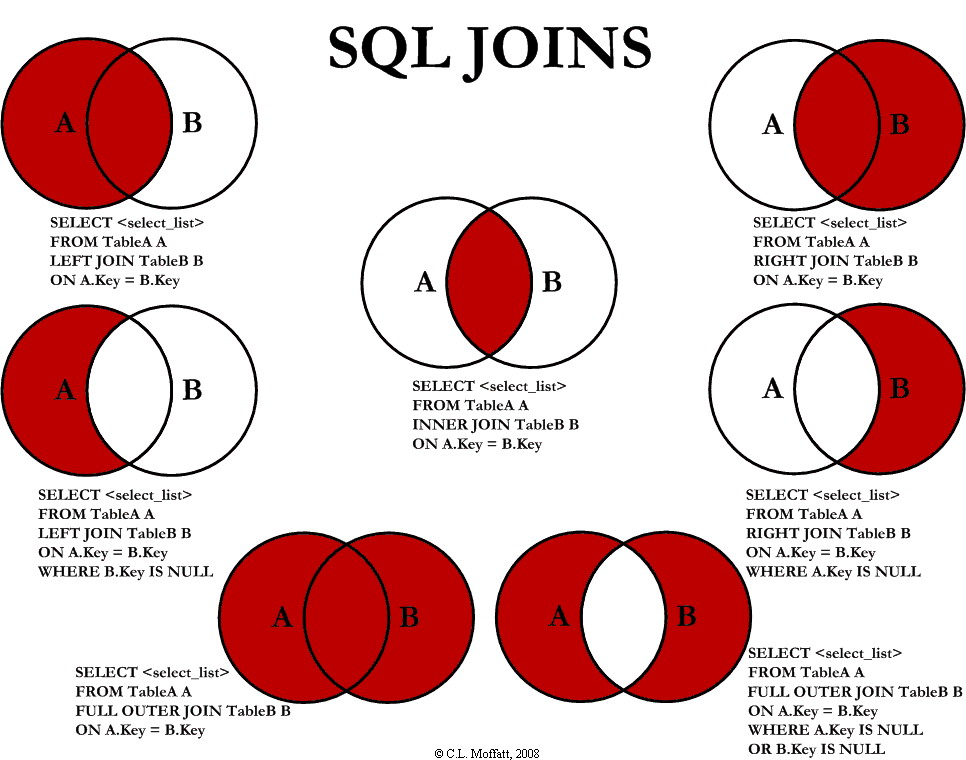
\includegraphics[width=1.00\linewidth]{SQLjoins}

\end{figure}

\end{frame}
\begin{frame}
	\frametitle{Joins}
Pretend data set listing country of origin for each species.
The variables ``Species" is common to both data frames.
	\begin{figure}
\centering
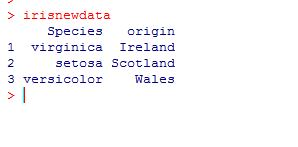
\includegraphics[width=0.7\linewidth]{irisnewdata}
\caption{Second Data Frame}
\label{fig:irisnewdata}
\end{figure}

\end{frame}

\begin{frame}
	\frametitle{Joins}
	\begin{figure}
\centering
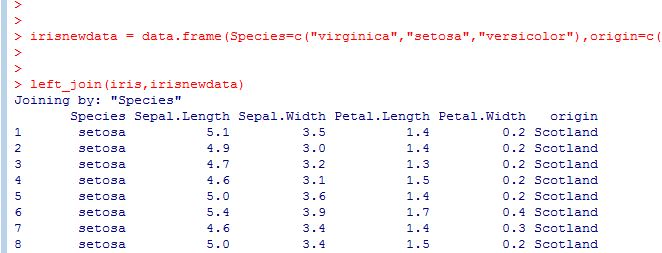
\includegraphics[width=0.97\linewidth]{irisjoin}

\label{fig:irisjoin}
\end{figure}

\end{frame}
%======================================================================= %

\begin{frame}
\frametitle{Set Theory Operations}

dplyr implements the methods for set theory operations

\begin{itemize}
	\item \texttt{intersect(x, y)}: all rows in both x and y
	\item \texttt{union(x, y)}: rows in either x or y
	\item \texttt{setdiff(x, y)}: rows in x, but not y
\end{itemize}
\end{frame}
\end{document}
